\documentclass{../Common/Structure/doc_pdf}

\titleSubtitle{{\Huge\textit{Power EnJoy}}\\{\LARGE Integration Test Plan Document}}{Version 1.0.0}
\pageHeader{Integration Test Plan Document}

\begin{document}
\titleToc
\newcommand{\testCase}[7]{%
	\unbreakableBlock{%
		\vspace{0.5em}
		\paragraphnewline{Test Case I#1}
		\newline
		\begin{tabulary}{\linewidth}{Y{3cm}|X{8.25cm}}
			\textbf{Test Item(s)} & #2 $\longleftrightarrow$ #3 \\ \hline
			\textbf{Input Specification} & #4 \\ \hline
			\textbf{Output Specification} & #5 \\ \hline
			\textbf{Environmental Needs} & #6 \\ \hline
			\textbf{Target} & #7 \\
		\end{tabulary}
		\vspace{0.5em}%	
	}%
}
\chapter{Introduction}
This document represent the Requirement Analysis and Specification Document (RASD). The main goal of this document is to completely describe the system in terms of functional and non-functional requirements, analyse the real need of the customer to modelling the system, show the constraints and the limit of the software and simulate the typical use cases that will occur after the development. This document is intended to all developer and programmer who have to implement the requirements, to system analyst who want to integrate other system with this one, and could be used as a contractual basis between the customer and the developer.
\section{List of definitions and abbreviations}
\paragraph{Definitions}
In the document are often used some specific terms whose definitions are reported bellow:
\begin{itemize}
	\item Server Database: data layer
	\item Server Application: application layer
	\item Client: client layer
	\item Mobile App: \textit{myTaxiService} mobile application, in Client
	\item Web App: \textit{myTaxiService} web application, in Client
	\item System: the union of software and hardware to be developed and implemented
	\itemBold{Integration Test Case} An atomic procedure done to test the integration of a component on the top of another one.
	\itemBold{Integration Test Suite} A collection of \textbf{Integration Test Cases}.
	\item See the correspondent section in the \textbf{RASD} and the \textbf{DD} for more definitions.
\end{itemize}
\paragraph{Acronyms}
\begin{itemize}
	\itemBold{RASD Requirements Analysis and Specification Document
	\itemBold{DD} Design Document
	\itemBold{API} Application Programming Interface
	\itemBold{DBMS} DataBase Management System
	\itemBold{ITPD} Integration Test Plan Document.
	\itemBold{In} Integration Test Suite number n.
	\itemBold{InTm} Integration Test Case number m of the Integration Test Suite number n.
	\itemBold{JS} JavaScript.
	\itemBold{UI} User Interface.
	\item See the correspondent section in the \textbf{RASD} and the \textbf{DD} for more acronyms and abbreviations.
\end{itemize}

\section{List of reference documents}
\begin{itemize}
	\item Software Engineering 2 Project AA 2016/2017: Project Description And Rules and Assignment 4 - integration test plan
	\item PowerEnJoy's Requirement Analysis and Specification Document (RASD)
	\item PowerEnJoy's Design Document (DD)
\end{itemize}
\newpage

\chapter{Integration Strategy}
\section{Entry Criteria}
Before starting the integration testing of any software component that has been designed for \PowerEnJoy{} system, the internal functions of the considered component (i.e. public or protected methods that are exposed within the package of the component but are not part of any external public interface) must be unit tested using an appropriate framework.
\section{Elements to be integrated}
\PowerEnJoy{} as shown in the \textbf{DD} is a three-tier system composed by:
\begin{itemize}
	\itemBold{DBMS} The memory of \PowerEnJoy{} entire system
	\itemBold{PowerEnJoy System} The main server and the main core composed by:
		\begin{enumerate}
			\item Data Manager
			\item Account Manager
			\item Ride Manager
			\item Bill Manager
			\item Map Services
			\item Notification
			\item Car Manager
			\item Zone Manager
			\item Problem Manager
		\end{enumerate}
	\itemBold{Client Application} Subdivided in \textbf{Car System} and \textbf{Mobile Application}
\end{itemize}
Moreover we assume that that Google Maps API and Paypal are well tested by their owner and thus we can use them without testing any further.

\section{Integration testing strategy}
The integration testing strategy, conducted in this project, is a \textbf{bottom-up} approach. This strategy tests the lower level components and start testing a way upwards to higher level components. The advantage of this strategy is that allow us to maintain the code easier, smaller modules have unit tests and there is a clearer structure of how to do things. The disadvantage is that when releasing a prototype it's impossible to see a working prototype until nearly all the program has been completed so that may take a long time before this happens. In early development, testing tools as Mockito and Arquillian (described in Chapter 4) allow us to test components which depend on incomplete ones through stubs and drivers (Chapter 5). The usage of the selected approach will create a robust application with efforts concentrated in testing the Server parts before all. 
%probably the component view needs to be changed in DD
\section{Sequence of component/function integration}
\subsection{Software integration sequence}
The following diagram illustrates the integration sequence of the various components, following the integration testing strategy described above. This means that in each subsystem, components are integrated starting from the most independent to the less independent, in order to prompt the chosen approach and improving modularity. 
\begin{center}
	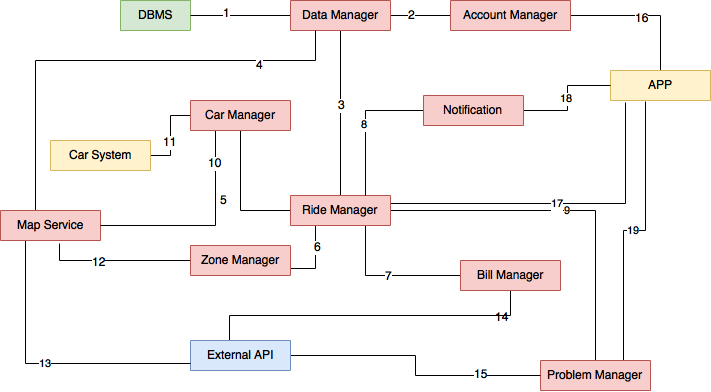
\includegraphics[width=\textwidth]{Diagrams/SoftwareIntegrationDiagram.png}
	\captionof{figure}{Software Integration Diagram}
	\label{Software Integration Diagram}
\end{center}

\subsection{Subsystem integration sequence}
The following diagram illustrates the integration sequence of the various subsystems, following the integration testing strategy described above. In particular, the Server Database is integrated before the Client, because the former does not need an actual functioning system in order to be tested efficiently, contrary to the latter.
%Image
\begin{center}
	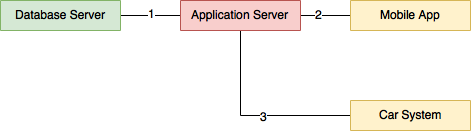
\includegraphics[width=\textwidth]{Diagrams/SubsystemsIntegrationDiagram.png}
	\captionof{figure}{Subsystem Integration Diagram}
	\label{Subsystem Integration Diagram}
\end{center}

\chapter{Individual steps and test description}
\subsection{Model Integration Test Cases}
\testCase
	{1}
	{Data Manager}
	{Account Manager}
	{A set of methods calls on Data Manager to retrieve user information}
	{Check if the user's information are correct}
	{Glassfish Server, a test Database, I1 successful}
	{Verify that the user information are retrieved from the Data Manager}

\testCase
	{2}
	{Data Manager}
	{Ride Manager}
	{A set of methods calls on Data Manager to retrieve reserved ride information}
	{Check if the user's information are correct}
	{Glassfish Server, a test Database, I1 successful}
	{Verify that the reserved ride info are retrieved from the Data Manager}
	
\testCase
	{3}
	{Data Manager}
	{Map Service}
	{A set of methods calls on Data Manager to retrieve informations about coordinates}
	{Check if the user's information are correct}
	{Glassfish Server, a test Database, I1 successful}
	{Verify that the info of coordinates are retrieved from the Data Manager}

\testCase
	{4}
	{Ride Manager}
	{Car Manager}
	{A set of methods calls on Car Manager}
	{Check if an available Car is returned}
	{Ride/Notification and Data/Account satisfied}
	{Retrieve an available Car}

\testCase
	{5}
	{Ride Manager}
	{Zone Manager}
	{A set of methods calls on Zone Manager}
	{Verify that the returned zone is the correct one}
	{Map Service/EXTApi and Car mng/Ride satisfied}
	{Find the position in a certain zone}

\testCase
	{6}
	{Ride Manager}
	{Bill Manager}
	{A set of methods calls on Bill Manager}
	{Verify that the total amount is correct}
	{Map/EXTApi, CarManager/System and Data/Account satisfied}
	{Verify that the Bill Manager calculate the correct amount of the ride}

\testCase
	{7}
	{Ride Manager}
	{Notification}
	{A set of methods calls in order to create a Notification}
	{Check if the correct notification is created}
	{Data/Account and Ride/Car satisfied}
	{Verify that the Notification Manager creates the notification from the Ride Manager}
	
\testCase
	{8}
	{Ride Manager}
	{Problem Manager}
	{A set of methods calls on Problem Manager}
	{Verify that the problem belong to the provided list}
	{Data/Account and Notification/Mobile satisfied}
	{Check if Problem Manager can handle correctly the calls, returning an element belong to the provided listbox}
	
\testCase
	{9}
	{Map Service}
	{External API}
	{Create a typical set of methods calls by Map Service on External API}
	{Check if all the methods of External  APIs Manager produce the expected results}
	{N/A}
	{Verify that the External APIs Manager works  with the Map Services Manager}
	
\testCase
	{10}
	{Bill Manager}
	{External API}
	{Create a typical set of methods calls by Bill Manager on External API}
	{Check if all the methods of External   APIs Manager produce the expected results}
	{N/A}
	{Verify that the External APIs Manager works  with the Bill Manager}

\testCase
	{11}
	{Problem Manager}
	{External API}
	{Create a typical set of methods calls by Problem Manager on External API}
	{Check that all the methods of External   APIs Manager produce the expected results}
	{N/A}
	{Verify that the External APIs Manager works  with the Problem Manager}

\testCase
	{12}
	{Car Manager}
	{Map Service}
	{A set of methods calls on Map Services Manager}
	{Verify that the position of the car is correct}
	{Map/EXT and Data/Account succesful}
	{Retrieve the position of a car in a certain position on the map}

\testCase
	{13}
	{Car Manager}
	{Car System}
	{A set of methods calls Car Manager}
	{Verify if the state of the car is correct}
	{Car with GPS and Data Connection enabled}
	{Verify that the information exchanged between car and system works}

\testCase
	{14}
	{Database Server}
	{Application Server}
	{Queries on the DBMS for the table Driver, Car, Ride and Zone}
	{The queries return the expected results}
	{Glassfish Server, a test Database}
	{Verify that the typical queries to the DBMS  works}

\testCase
	{15}
	{Application Server}
	{Mobile App}
	{A set of methods calls on both Server Application and Mobile App }
	{Check if methods calls mentioned in Input Specification produce the expected results}
	{Glassfish, a test Database}
	{Verify the interaction between Server Application and Mobile App works}

\testCase
	{16}
	{Mobile App}
	{Account Manager}
	{Create a typical set of methods calls performed by Mobile App on Account Manager}
	{Check if methods calls mentioned in Input Specification produce the expected results}
	{A device that can run Mobile App}
	{Verify  if Account Manager can handle correctly Mobile App methods calls}
	
\testCase
	{17}
	{Mobile App}
	{Ride Manager}
	{Create a typical set of methods calls performed by Mobile App on Ride Manager}
	{Check if methods calls mentioned in Input Specification produce the expected results}
	{A device that can run Mobile App}
	{Verify  if Ride Manager can handle correctly Mobile App methods calls}

\testCase
	{19}
	{Mobile App}
	{Notification}
	{Create a typical set of methods calls performed by Mobile App on Notification}
	{Check that methods calls mentioned in Input Specification produce the expected results}
	{A device that can run Mobile App}
	{Verify  if Notification can handle correctly Mobile App methods calls}

\chapter{Tools and test equipment required}
%TODO Identify all tools and test equipment needed to accomplish the integration. Refer to the tools presented during the lectures. Explain why and how you are going to use them. Note that you may also use manual testing for some part. Consider manual testing as one of the possible tools you have available.
The following part of the document contains a set of recommended software that can be used to implement the concrete procedure of testing.
Moreover, because the high-level architecture proposed in the \textbf{DD} is designed using a \textbf{Java-based} style, the programming language that better adapts to this style is \textbf{Java}, but a lot of other emerging languages can be used in order to build a proper software, like \textbf{Swift}.\par
If it is decided to use \textbf{Java}, the proposed and well-known tools are:
\begin{itemize}	
	\itemBold {JUnit} Unit testing framework.
	\begin{itemize}
		\item 
		\href{http://junit.org/}{http://junit.org/}
	\end{itemize}	
	\itemBold{Mockito} Another unit testing framework.
	\begin{itemize}
		\item 
		\href{http://site.mockito.org/}{http://site.mockito.org/}
	\end{itemize}	
	\itemBold {Arquillian} Integration testing framework.
	\begin{itemize}
		\item \href{http://arquillian.org/}{http://arquillian.org/}
	\end{itemize}
	\itemBold {Espresso} Android UI testing automation.
	\begin{itemize}
		\item \href{http://developer.android.com/training/testing/ui-testing/espresso-testing.html}{http://developer.android.com/training/testing/ui-testing/espresso-testing.html}
	\end{itemize}
\end{itemize}
%TO it for swift

\chapter{Program stubs and test data required}
This section describes the specification of stubs and drivers needed to replace the part of software components that still don?t exist and test the others. This is necessary to perform the integration steps. DBMS should contain sample data in order to perform proper test cases. We assume that the \textbf{Integration testing} comes after \textbf{Developing} and \textbf{Unit testing}. In this way we don't need any \textbf{Driver} because the software components are already developed.\par
On the other hand we need few \textbf{Stubs} in order to make the not yet integrated components work, because we want to respect the \textbf{Bottom-Up} strategy.\par
To better catch the need for introducing \textbf{Stubs}, an example of a specific \textbf{Stub} usage is proposed below.\par
In order to integrate the \textbf{Map Service} in \textbf{I9} we need a component that mocks \textbf{Map Service} functionalities in a predefined way. 
To respect the \textbf{Bottom-Up} strategy, given the fact that the \textbf{TD Locator} is a component of the \textbf{TD View}, we have decided to introduce its \textbf{Stub}.
The real \textbf{Map Service} will be integrated when the integration procedure arrives to \textbf{Map Service}.\par
In \textbf{I1} there is the need for some sample data to be in the \textbf{Database}, and in \textbf{I13} some sample GPS data are needed.


\appendix
\chapter{Appendix}

\section{Tools}
\begin{itemize}
	\itemBold{TeXstudio} \LaTeX{} editor used to write the document.
	\itemBold{StarUML} To draw diagram.\end{itemize}
\section{Hours of work}
In the following are listed the hours of work that each member of the group did:
\begin{enumerate}
	\item Marco Redaelli: 19 \emph{hours}
	\item Francesco Zanoli: 19 \emph{hours}
\end{enumerate}
\section{Version History}
In the following are listed the differences between versions:
\begin{enumerate}
	\itemBold{ 15/01/2017} First version
\end{enumerate}

\end{document}
